\documentclass{standalone}
\usepackage{tikz}
\begin{document}
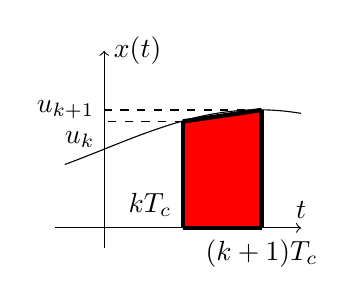
\begin{tikzpicture}[scale=2.5]
    \draw[fill=red](0.4,1.141)--(0.8,1.199)--(0.8,0.6)--(0.4,0.6)--(0.4,1.141);

    \draw[->](0,0.5)--(0,1.5)node[right]{$x(t)$};
    \draw[->](-0.25,0.6)--(1,0.6)node[above]{$t$};

    \draw[]plot[smooth, domain=-0.2:1](\x,{1+0.2*sin(2*\x r)});
    %\draw[->,ultra thick](0,0)node[below left]{$0$}--(0,1);
    \draw[-,ultra thick](0.4,0.6)node[above left]{$kT_c$}--(0.4,1.141);
    \draw[-,ultra thick](0.8,0.6)node[below]{$(k+1)T_c$}--(0.8,1.199);
    \draw[-,ultra thick](0.4,1.141)--(0.8,1.199);
    \draw[-,ultra thick](0.4,0.6)--(0.8,0.6);


    \draw[dashed](0.4,1.141)--(0,1.141)node[below left]{$u_k$};
    \draw[dashed](0.8,1.199)--(0,1.199)node[left]{$u_{k+1}$};
\end{tikzpicture}
\end{document}